\documentclass[addpoints]{exam}
\usepackage[utf8]{inputenc}


\usepackage{hyperref}
\hypersetup{
    colorlinks=true,
    linkcolor=blue,
    filecolor=magenta,      
    urlcolor=cyan,
}


\usepackage{pdfsync}
\usepackage{fontspec}
\usepackage[T1]{fontenc}
\usepackage[utf8]{inputenc}
\usepackage{etoolbox}
\usepackage{tikz}
\usepackage{pgfplots}
\usepackage{subfig}
\usepackage{tikzscale} % Scale the figure not the font
\tikzset{
font={\fontsize{5pt}{5}\selectfont}}
\usepackage{tikzscale} % Scale the figure not the font
\usepackage{textpos}
\usepackage{standalone}
\usepackage{color}
\pgfplotsset{tick scale binop=\times}
\usepackage{tikz-dimline}
\usepackage[skins,theorems]{tcolorbox}
\usepackage{animate}


\usepackage{amsmath}
\usepackage{booktabs}
\usepackage{cancel}
\usepackage{caption}
\usepackage{cleveref}
\usepackage{colortbl}
\usepackage{csquotes}
% \usepackage{helvet}
% \usepackage{millennial}
\usepackage{multirow}
\usepackage{listings}
\usepackage{xcolor}

\usepackage{esint} % various fancy integral symbols
\usepackage{outlines}



\usepackage{physics} % For using the oridnary derivative
\usepackage{siunitx}
\sisetup{per=slash, load=abbr, output-complex-root = j, complex-root-position = before-number, round-mode=figures,round-precision=4}

%% Tikz Libraries
\usetikzlibrary{positioning}
\usetikzlibrary{arrows}
\usetikzlibrary{patterns}
\usetikzlibrary{backgrounds}
\usetikzlibrary{calc}
\usetikzlibrary{decorations.pathreplacing}



\newcommand{\ti}[1]{\tilde{#1}} % spectral representation
\newcommand{\tnsr}[1]{\underline{\underline{#1}}}

% Symbols
\renewcommand{\O}{\omega}  % omega
\newcommand{\E}{\varepsilon}  % epsilon
\renewcommand{\u}{\mu}  % mu
\newcommand{\p}{\rho}  % rho
\newcommand{\x}{\times}  % times
\renewcommand{\inf}{\infty}  % infinity
\newcommand{\infint}{\int\limits_{-\inf}^\inf} % integral by R
\newcommand{\e}{\mathrm{e}} % Straight-up exponential
\renewcommand{\j}{{j}\mkern1mu} % Straight-up exponential
\newcommand{\iu}{\mathrm{i}\mkern1mu}

\newcommand\ddfrac[2]{\frac{\displaystyle #1}{\displaystyle #2}}

\title{High Frequency Communication Systems}
\author{Homework 7 - Antenna Arrays - Analysis and Design}
\date{Semester 2, 2020/21}

\begin{document}

\maketitle


\begin{questions}
    \pointsinrightmargin 
    \bracketedpoints

\question[5] Plot the array factor for an \textit{ordinary} endfire array which is uniformly excited, and contains five elements with spacings $d = 0.35 \lambda$. Consider the main direction of radiation, $\theta_0 = \ang{180}$. Sketch as well as plot using a computer program the radiation pattern of the array. 

\question Design a six element antenna array with a design requirement of $\text{SLL} = 0$ and the main beam in the endfire direction $\theta_0 = \ang{0}$. 
\begin{parts}
    \part[5]
    For the element spacing of $d = 0.25 \lambda$, find and plot the radiation pattern, and calculate the first null beamwidth (BWFN).
    \part[3]
    Repeat for $d = 0.40 \lambda$
    \part[2] For an application requiring higher directivity, which array configuration is better?
    \end{parts}


\question[5]

For the array configuration as shown in Fig. \ref{fig:arrays}, find and plot the radiation pattern. 

\begin{figure}[htbp]
    \centering
    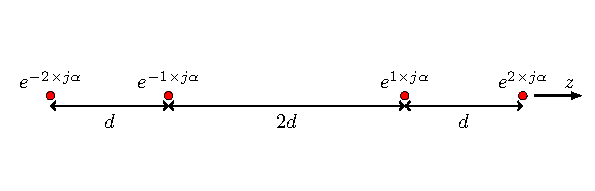
\includegraphics[width=0.75\textwidth]{5_elements.pdf}
    \caption{Antenna Array Configuration.}
    \label{fig:arrays}
\end{figure}
\end{questions}

\end{document}

